Consider an op amp having a single pole open loop response $G_{0} = 10^5$ and $f_{p} = 10$ Hz.  Let the OPAMP be ideal connected in non-inverting terminal with a nominal low frequency of closed loop gain of 100 
\begin{enumerate}
\item A manufacturing error introducing a second pole at $10$ kHz. Find the frequency at which $\abs{GH} = 1$ and the corresponding phase margin.
\item For what values of $H$ is the phase margin greater than 45\degree ?
\end{enumerate}
\begin{enumerate}[label=\arabic*.,ref=\theenumi]
%\begin{enumerate}[label=\thesubsection.\arabic*.,ref=\thesubsection.\theenumi]
\numberwithin{equation}{enumi}

\item Find the transfer function of the two pole OPAMP.

\solution 
For a two-pole amplifier open loop transfer function is 

\begin{align}
    G\brak{s} = \frac{G_{0}}{\brak{1+\frac{s}{\omega_{1}}}\brak{1+\frac{s}{\omega_{2}}}}
\end{align}
Poles are at $f_{1} =10$ and $f_{2} = 10^{4}$
\begin{align}
G\brak{f} &= \frac{G_{0}}{\brak{1+\j\frac{f}{f_{1}}}\brak{1+\j\frac{f}{f_{2}}}}
\\
&= \frac{10^{5}}{\brak{1+\j\frac{f}{10}}\brak{1+\j\frac{f}{10^{4}}}}
\label{eq:ee18btech11034_1}
\end{align}
\item Find the feedback $H$.
\\
\solution  Since the closed loop gain 
\begin{align}
    \abs T = 100
\end{align}
and for nominal low frequency $\abs{GH} \gg 1$,
\begin{align}
    H &\approx  \frac{1}{\abs{T}}= 0.01
    \label{eq:ee18btech11034_2}
\end{align}
\item Find the PM and the crossover frequency.
\\
\solution 
%For the $|GH| = 1$ and 
From \eqref{eq:ee18btech11034_1} and \eqref{eq:ee18btech11034_2}
\begin{align}
\abs{GH} &= 1
\\
\implies    \frac{10^{3}}{\brak{\sqrt{1+\frac{f^2}{100}}}\brak{\sqrt{1+\frac{f^2}{10^{8}}}}} &= 1
\\
\text{or } f_{180} &= 7.8615 \, kHz. 
%\end{align}
%\begin{align}
%    \brak{1+\frac{f^2}{100}}\brak{1+\frac{f^2}{10^{8}}} = 10^{6}
%\end{align}
%Solving f using python code  
%\begin{align}
%    f = 
\end{align}
using the following python code.
\begin{lstlisting}
codes/ee18btech11034/ee18btech11034.py
\end{lstlisting}
From \eqref{eq:ee18btech11034_1}, $\because \phase{H} = 0\degree$,
\begin{align}
\label{eq:ee18btech11034_phaseGH}
\phase{G(f)H(f)} &= \phase{G(f)}
\\
&-\tan^{-1}\brak{\frac{f}{10}} -\tan^{-1}\brak{\frac{f}{10^{4}}}
\\
\implies PM &= 180 \degree + \phase{G(f_{180})} 
\\
&= 180 \degree -128.1 \degree = 51.9 \degree
\end{align}
%At $f = 7861.5$
%\begin{align}
%    \phi = -128.1\degree
%    \\
%    \implies \alpha = 180\degree + \phi
%    \label{eq:ee18btech11034_3}
%    \\
%    \implies \alpha = 51.9\degree
%\end{align}

\item Verify your result using a Bode plot.
\\
\solution  The following code  generates Fig. \ref{fig:ee18btech11034_1}

\begin{lstlisting}
codes/ee18btech11034/ee18btech11034_1.py
\end{lstlisting}
%
\begin{figure}[!h]
\centering
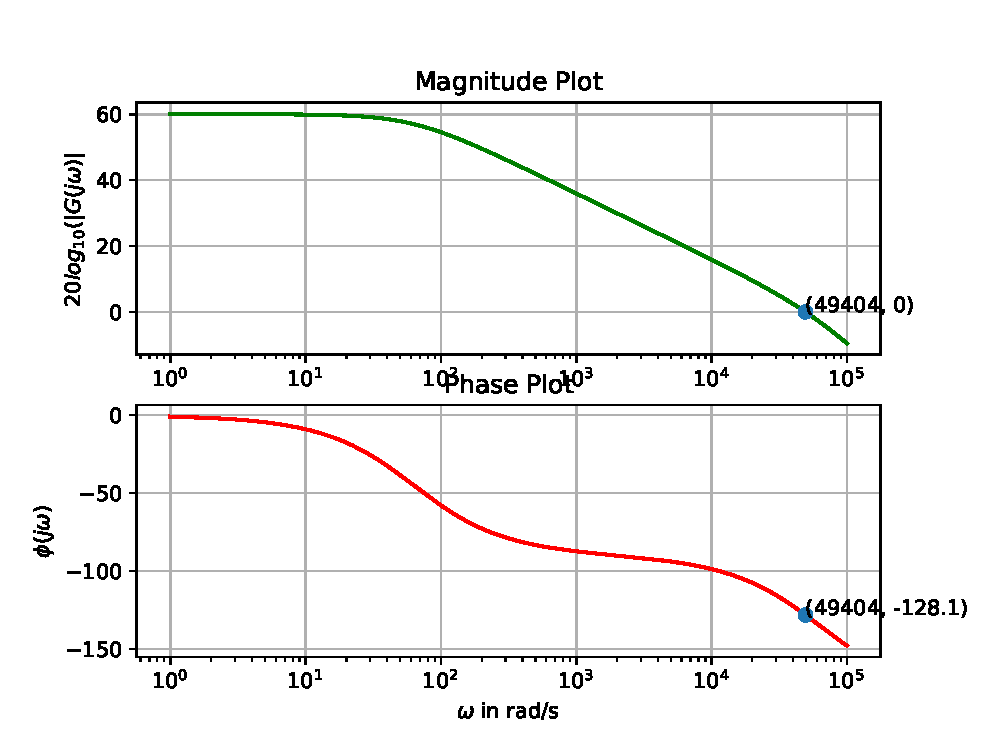
\includegraphics[width=\columnwidth]{./figs/ee18btech11034/ee18btech11034_1.eps}
\caption{}
\label{fig:ee18btech11034_1}
\end{figure}
%

\item Realise the above system with $PM = 51.9 \degree$ using a feedback circuit.\\
\solution
\begin{figure}[ht!]
	\begin{center}
		\resizebox{\columnwidth/1}{!}{\begin{circuitikz}[american]
\ctikzset{tripoles/mos style/arrows}
\draw (1,2) to[short, -o] (0,2) node[label={above:$V_{in}$}]{};
\draw (1,2) to[R=$R$, i=$I$] (3,2) to[C=$C$] (3,0) node[ground](GND){};
\draw (3,2) to[short, -o] (4,2) node[label={above:$V_{out}$}]{};
\end{circuitikz}
}
	\end{center}
	\caption{}
	\label{fig:ee18btech11034_figa}
\end{figure}

The transfer function of OPAMP is
\begin{align}
    G\brak{s} = \frac{10^{5}}{\brak{1+\frac{s}{2\pi \times 10}}\brak{1+\frac{s}{2\pi \times 10^{4}}}}
\end{align}
%
\item For the feedback gain H\\
\solution\\
Choose a resistance network such that
\begin{align}
    H = \frac{V_{f}}{V_{o}} = \frac{R_{1}}{R_{1}+R_{2}} \approx 0.01
\end{align}
\begin{figure}[ht!]
	\begin{center}
		\resizebox{\columnwidth}{!}{\begin{circuitikz}[american]

\draw (2,2)  node[op amp] (OA) {};
\draw (OA.+) -- (0,1.5) to[vsourcesin, l= $V_{s}$] (0,0) node[ground](GND){};
\draw (OA.-) -- (0,2.5) node[ground, rotate=270](GND){};
\draw (OA.out) -- (3,2) node[label={above:$V_{p}$}]{};
\draw (3,2) to[R=$5300\ohm$] (5.5,2) node[label={}]{} to[C,l_=$3nF$] (5.5,0) node[ground](GND){};
\draw (5.5,2) -- (6.5,2) node[label={above:$V_{o}$}]{};

\end{circuitikz}
}
	\end{center}
	\caption{}
	\label{fig:ee18btech11034_figb}
\end{figure}

Choose $R_{1}$ and $R_{2}$ as
\begin{align}
    R_{1} = 10\ohm\\
    R_{2} = 990\ohm
\end{align}
\begin{align}
H = \frac{R_{1}}{R_{1}+R_{2}} = \frac{10}{10+990} = 0.01
\end{align}
\item Feedback Circuit for $PM = 51.9\degree$
\\
\solution
\begin{figure}[ht!]
	\begin{center}
		\resizebox{\columnwidth}{!}{\begin{circuitikz}[american]
\ctikzset{tripoles/mos style/arrows}
\draw (1,2) to[short, -o] (0,2) node[label={above:$V_{o}$}]{};
\draw (1,2) to[R=$1000\ohm$] (2,2) -- (3,2) to[R=$10\ohm$] (3,0) node[ground](GND){};
\draw (3,2) to[short, -o] (4,2) node[label={above:$V_{f}$}]{};
\end{circuitikz}
}
	\end{center}
	\caption{}
	\label{fig:ee18btech11034_figc}
\end{figure}

\item Verification using spice simulation\\
\solution For $H=0.01$ the closed loop response is
\begin{align}
\abs T \approx \frac{1}{H} = 100
\end{align}
The following is the netlist file for spice
\begin{lstlisting}
spice/ee18btech11034/ee18btech11034_1.net
\end{lstlisting}
\begin{figure}[!h]
\centering
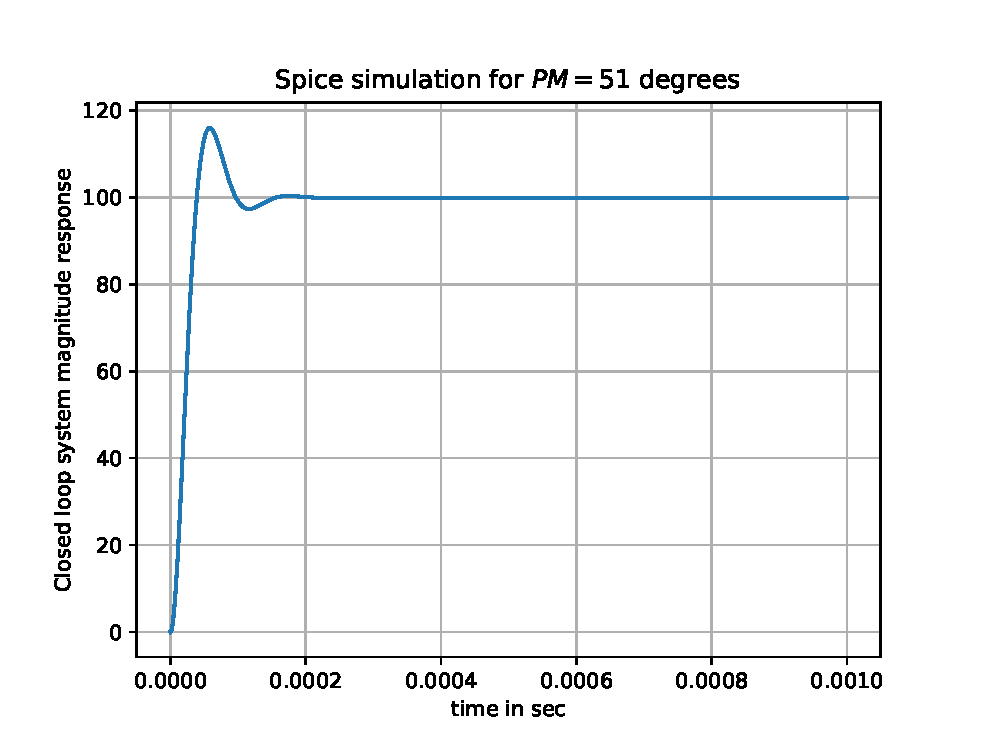
\includegraphics[width=\columnwidth]{./figs/ee18btech11034/ee18btech11034_spice_result1.eps}
\caption{}
\label{fig:ee18btech11034_spice_result1}
\end{figure}
The following python code plots the closed loop response verses time
\begin{lstlisting}
spice/ee18btech11034/ee18btech11034_spice_result1.py
\end{lstlisting}
%
\item Find $H$ such that $PM = 45\degree$.
\\
\solution From \eqref{eq:ee18btech11034_phaseGH},
assuming constant $H$,
\begin{align}
\phase{G(f_{180})} = 45\degree - 180 \degree &=  -135\degree
\\
\implies -\tan^{-1}\brak{\frac{f}{10}} -\tan^{-1}\brak{\frac{f}{10^{4}}}  &= -135\degree
\\
\implies     \frac{\frac{f}{10} + \frac{f}{10^{4}}}{1-\frac{f^2}{10^{5}}} &= -1
\\
\text{or, }    f_{180} \approx 10 \, kHz
\end{align}
From \eqref{eq:ee18btech11034_1},
\begin{align}
\because  \abs{G\brak{f_{180}}H}&=1,
\\
  \frac{\brak{10^{5}}H}{\brak{\sqrt{1+\frac{10^{8}}{100}}}\brak{\sqrt{1+\frac{10^{8}}{10^{8}}}}} &= 1
\\
\implies     H &= 1.414 \times 10^{-2}
    \\
  \text{or, }  H_{max} =  1.414 \times 10^{-2}
\end{align}
which is the value of $H$ for which $PM > 45\degree$.

\item Verify the above using a Bode plot. 
\\
\solution 
The following code plots  Fig. \ref{fig:ee18btech11034_2}.
%
\begin{lstlisting}
codes/ee18btech11034/ee18btech11034_2.py
\end{lstlisting}
%
\begin{figure}[!h]
\centering
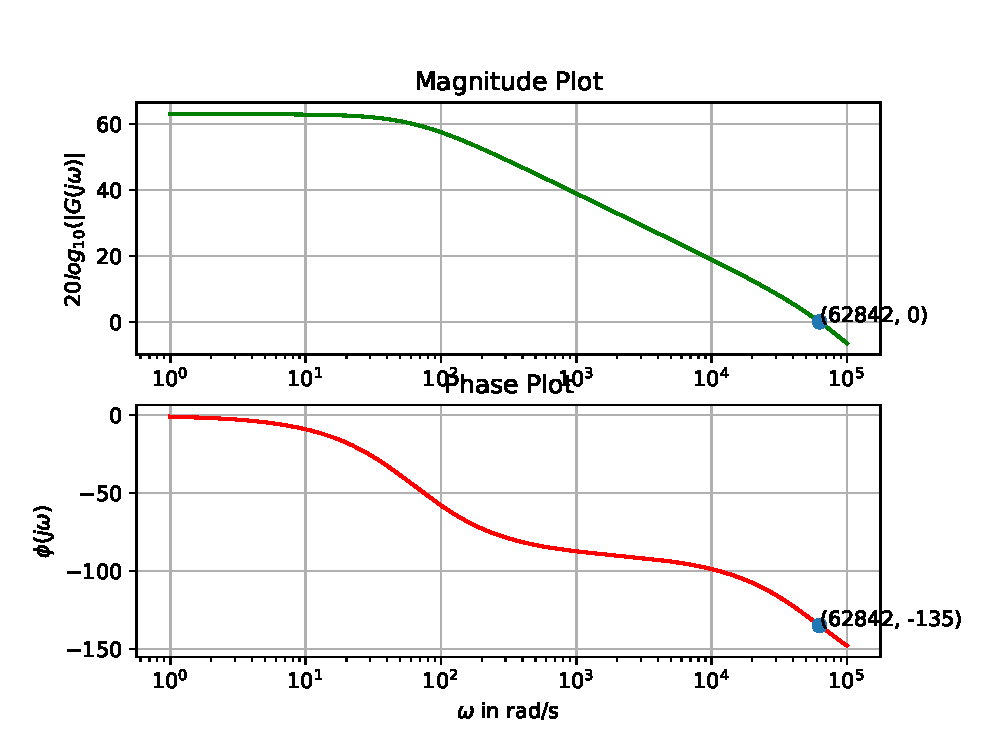
\includegraphics[width=\columnwidth]{./figs/ee18btech11034/ee18btech11034_2.eps}
\caption{}
\label{fig:ee18btech11034_2}
\end{figure}
The transfer function of OPAMP will be unchanged.
For the required feedback gain H the feedback circuit changes

\item Realise the above system with $PM = 45 \degree$ using a feedback circuit.\\
\solution
\begin{figure}[ht!]
	\begin{center}
		\resizebox{\columnwidth}{!}{\tikzstyle{block} = [draw, rectangle, 
    minimum height=1.25em, minimum width=2.5em]
\tikzstyle{sum} = [draw, circle, node distance=1cm]
\tikzstyle{input} = [coordinate]
\tikzstyle{output} = [coordinate]
\tikzstyle{pinstyle} = [pin edge={to-,thin,black}]

% The block diagram code is probably more verbose than necessary
\begin{tikzpicture}[auto, node distance=2.5cm,>=latex']
    % We start by placing the blocks
    \node [input, name=input] {};
    \node [sum, right of=input] (sum) {};
    \node [block, right of=sum] (controller) {$\frac{10^{5}}{\brak{1+\frac{s}{2\pi \times 10}}\brak{1+\frac{s}{2\pi \times 10^{4}}}}$};
    
    % We draw an edge between the controller and system block to 
    % calculate the coordinate u. We need it to place the measurement block. 
   
    \node [output, right of=controller] (output) {};
    \node [block, below of=controller] (measurements) {$1.414 \times 10^{-2}$};

    % Once the nodes are placed, connecting them is easy. 
    \draw [draw,->] (input) -- node[pos=0.99] {$+$} node {$V_{s}$} (sum);
    \draw [->] (sum) -- node {$V_{i}$} (controller);
    \draw [->] (controller) -- node [name=y] {$V_{o}$}(output);
    \draw [->] (y) |- (measurements);
    \draw [->] (measurements) -| node[pos=0.99] {$-$} node [near end] {$V_{f}$} (sum);
\end{tikzpicture}}
	\end{center}
	\caption{}
	\label{fig:ee18btech11034_figd}
\end{figure}

\item For the feedback gain H\\
\solution
\begin{align}
    R_{1} = 10\ohm
\end{align}
\begin{align}
    R_{2} = 700\ohm
\end{align}
\begin{align}
    H = \frac{R_{1}}{R_{1}+R_{2}} 
    \implies \frac{10}{10+700} \approx 1.41 \times 10^{-2}
\end{align}

\item Feedback Circuit for $PM = 45\degree$\\
\solution
\begin{figure}[ht!]
	\begin{center}
		\resizebox{\columnwidth}{!}{\begin{circuitikz}[american]

\draw (2,2)  node[op amp] (OA) {};
\draw (OA.+) -- (0,1.5) to[vsourcesin, l= $V_{s}$] (0,0) node[ground](GND){};
\draw (OA.-) -- (0,2.5) node[label={below:$V_{f}$}]{} to[R,l_=$14\ohm$] (-2,2.5) node[ground](GND){};
\draw (OA.out) -- (3,2) node[label={above:$V_{p}$}]{};
\draw (3,2) to[R=$5300\ohm$] (5.5,2) node[label={}]{} to[C,l_=$3nF$] (5.5,0) node[ground](GND){};
\draw (5.5,2) -- (6.5,2) node[label={above:$V_{o}$}]{};
\draw (5.5,2) -- (5.5,4) to[R=$10^{3}\ohm$] (0,4) -- (0,2.5);
\end{circuitikz}
}
	\end{center}
	\caption{}
	\label{fig:ee18btech11034_fige}
\end{figure}
\item Verification using spice simulation\\
\solution For $H=0.014$ the closed loop response is
\begin{align}
\abs T \approx \frac{1}{H} = 70.72
\end{align}
The following is the netlist file for spice
\begin{lstlisting}
spice/ee18btech11034/ee18btech11034_2.net
\end{lstlisting}
\begin{figure}[!h]
\centering
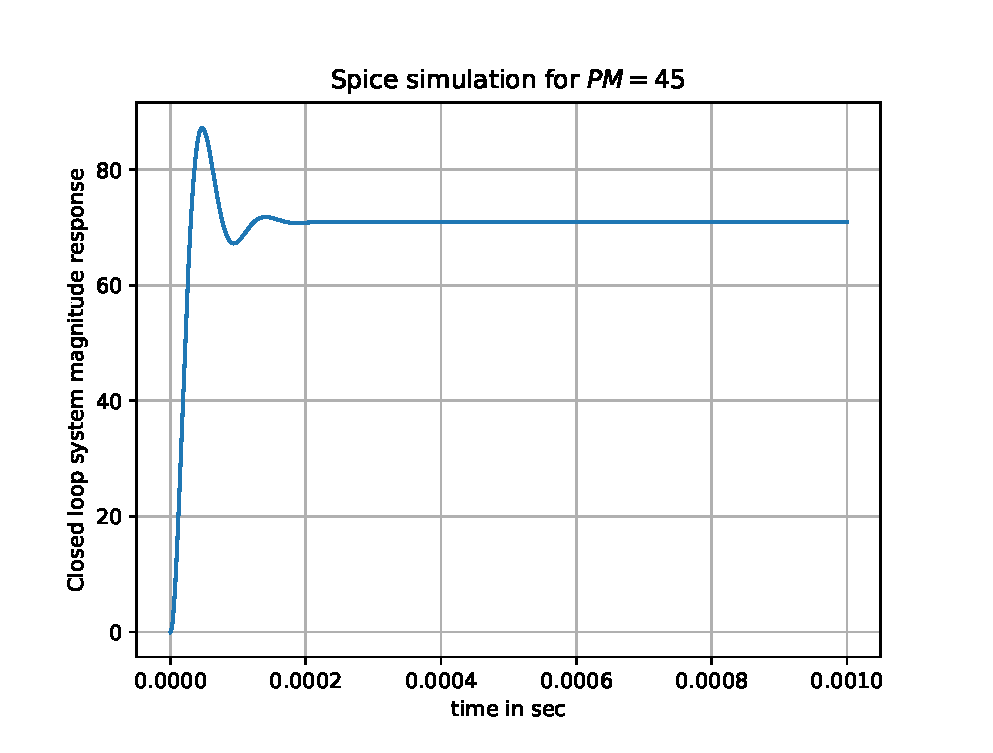
\includegraphics[width=\columnwidth]{./figs/ee18btech11034/ee18btech11034_spice_result2.eps}
\caption{}
\label{fig:ee18btech11034_spice_result2}
\end{figure}
The following python code plots the closed loop response verses time
\begin{lstlisting}
spice/ee18btech11034/ee18btech11034_spice_result2.py
\end{lstlisting}
\end{enumerate}
